\section{H : Constructed Types - $1D$ Arrays \& Structures }
\label{chap:contypes}

\begin{frame}[fragile]
\frametitle{{\em 1D} Arrays}
\begin{columns}

\begin{column}{0.55\textwidth}
\begin{itemize}
\item One-Dimensional arrays are declared by a type
followed by an identifier with a bracketed constant expression:
{\small
\begin{verbatim}
float x[10];
int k[ARRAY_SIZE];
float y[i*2];
\end{verbatim}
}
The following, however, is not valid:
{\small
\begin{verbatim}
float y[i*2];
\end{verbatim}
}
\item Arrays are stored in contiguous memory, e.g.:
{\small
\begin{verbatim}
int a[5];
\end{verbatim}
}
\begin{center}
\begin{figure}[h]
\centerline{
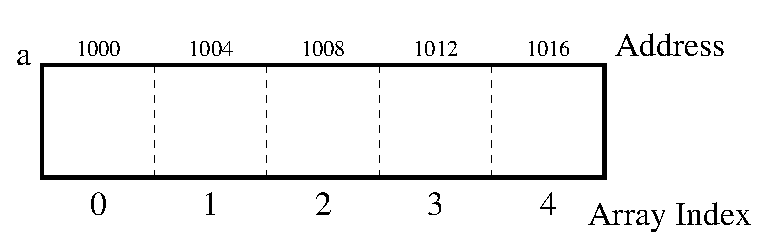
\includegraphics[scale=0.40]{../Figs/array9_1.eps}
}
\end{figure}
\end{center}
\item Arrays are indexed {\bf 0} to {\bf n-1}.
\end{itemize}
\end{column}

\begin{column}{0.35\textwidth}
\lstinputlisting[style=basicc]{../Code/ChapH/1d_array.c}
\end{column}

\end{columns}
\end{frame}



\begin{frame}[fragile]
\frametitle{{\em 1D} Arrays : Initialisation}
\begin{columns}

\begin{column}{0.45\textwidth}
By default, arrays are uninitialised.
When they are declared, they may be assigned a value:
{\small
\begin{verbatim}
float x[7] = {-1.1,0.2,2.0,4.4,6.5,0.0,7.7};
\end{verbatim}
}
or,
{\small
\begin{verbatim}
float x[7] = {-1.1, 0.2};
\end{verbatim}
}
the elements 2 ... 6 are set to zero.

Also:
{\small
\begin{verbatim}
int a[] = {3, 8, 9, 1};
\end{verbatim}
}
is valid, the compiler assumes the array size to be \verb^4^.
\end{column}

\begin{column}{0.45\textwidth}
\begin{itemize}
\item Accessing an array out of bounds will not be identified by
the compiler. It may cause an error at run-time.
One frequent result is that an entirely unrelated variable
is altered.
\item \verb^a[5] = a[4] + 1;^
\item \verb^k[9]++;^
\item \verb^n[12+i] = 0;^
\end{itemize}
\end{column}

\end{columns}
\end{frame}



\begin{frame}[fragile]
\frametitle{{\em 1D} Arrays : Call by Reference}
\begin{columns}

\begin{column}{0.35\textwidth}
\begin{itemize}
\item Here, the array is passed by {\em Reference} - no copy of
the array is made - the function processes the array that was created inside \verb^main()^, despite
it apparently having a `different' name.
\item All arrays are passed like this in C - we'll see later when we look at {\em pointers} why this is the case.
\end{itemize}
\end{column}

\begin{column}{0.55\textwidth}
\lstinputlisting[style=basicc]{../Code/ChapH/mean.c}
\end{column}

\end{columns}
\end{frame}




\begin{frame}[fragile]
\frametitle{Structures}
\begin{columns}

\begin{column}{0.45\textwidth}
\begin{itemize}
\item A structure type allows the programmer to aggregate components
into a single, named variable. Other languages call these {\it Records} or {\it Tuples}.
\item Each component has individually named members.
\item \begin{verbatim}
struct employee {
   long id;
   double salary;
   short age;
};
\end{verbatim}
\item \verb^struct^ is a keyword, \verb^employee^ is the structure
tag name, and \verb^id^, \verb^salary^ and \verb^age^ are members of the structure.
\end{itemize}
\end{column}

\begin{column}{0.45\textwidth}
\begin{itemize}
\item A statement of the form :\\
\verb^struct employee e1, e2;^\\
actually creates storage for the variables. 
\item A member is accessed using the member operator ``.''
\item
\begin{verbatim}
e1.salary = 35000.2;
e2.age = 29;
\end{verbatim}
\item The member name must be unique within the same structure.

\item Arrays of structures are possible, i.e.:
\begin{verbatim}
struct employee team[400];
\end{verbatim}
\end{itemize}
\end{column}

\end{columns}
\end{frame}

\begin{frame}[fragile]
\frametitle{Arrays of Structures}
\begin{columns}[T]

\begin{column}{0.45\textwidth}
\lstinputlisting[style=basicc,linerange={1-33},numbers=none]{../Code/ChapH/cards.c}
\end{column}

\begin{column}{0.45\textwidth}
\lstinputlisting[style=basicc,linerange={35-58},numbers=none]{../Code/ChapH/cards.c}
\end{column}

\end{columns}
\end{frame}

\begin{frame}[fragile]
\frametitle{Arrays of Structures}
\begin{columns}

\begin{column}{0.45\textwidth}
\lstinputlisting[style=basicc,linerange={60-95},numbers=none]{../Code/ChapH/cards.c}
\end{column}

\begin{column}{0.45\textwidth}
\outputlisting{../Code/ChapH/cards.autoout}
\begin{itemize}
\item The \verb^print_deck()^ function is clearly messy ! We can simplify this a little when we understand strings.
\end{itemize}
\end{column}

\end{columns}
\end{frame}
